\chapter{流式主题模型的实现}
\label{chapter:implement}
参数服务器的出现,使得分布式并行算法的实现更加简便高效。
目前已知的大规模高效主题模型算法的实现都采用了参数服务器\cite{li2014scaling}, 比如YahooLDA\cite{ahmed2012scalable}, LightLDA\cite{yuan2015lightlda}, 以及Peacock\cite{li2014scaling}(只实现了模型并行服务,还未抽象出来参数服务器)。
本章将介绍使用参数服务器来构建的流式主题参数数据结构,以及在此基础上的一些具体算法优化方案。

\section{参数服务器简介}
\subsection{数据并行}
数据并行指的是将数据进行分割,并分配给不同的计算节点并行地执行计算任务。
提及数据并行,我们往往能够想到Hadoop MapReduce和Spark等系统。

MapReduce通过简单的Mapper和Reducer的抽象提供的编程模型,可以在一个由几十到上百台的廉价机器集群上并发地,分布式地处理海量数据集,同时具有高可用性。
Spark则是一种内存的MapReduce扩展,Spark的核心数据结构是RDD(Resilient Distributed Dataset, RDD),该数据结构可以将数据持久化在内存中,从而避免了MapReduce不同阶段之间数据需要反复落盘的缺点。

这些系统允许一些严格同步的通信和迭代。借助这些大数据并行计算框架,有人开发了一些基于数据并行的机器学习库,比如Mahout\cite{mahout}, MLI\cite{sparks2013mli}。
这些算法库在小规模算法上效果尚可,一旦集群规模变大或者算法模型变大,算法执行过程中的需要大量的网络通信以及参数同步,网络的延迟和漫长的同步等待,会逐渐影响算法执行速度。

\subsection{模型并行}
模型并行指的是将大规模参数模型分布式地存储在不同机器节点上,并行地利用所有数据训练算法。
在算法训练过程中,每个分区会得到一部分参数子集的更新,在最终更新到模型之前通常会各个分区的结果进行合并。
这种方法使用于具有大规模参数的模型,同时数据量又不是特别大的场景。
这种时候算法执行过程中不会频繁地进行网络通信,同时算法的每个分区只会使用和更新一小部分参数子集。这种方法的优点是,算法同步的效率高,网络通信开销和延迟小。但是当数据规模太大时,每个工作结点可能无法完全加载所有的数据样本。

\subsection{参数服务器}
在现实业务场景中,机器学习算法的数据量可能会非常之大,这使得单机无法完全加载训练数据,同时也无法存储下来所有的参数。
通常的解决方案是数据并行或是模型并行,这两种方案在一些场景中非常有用。
但是还有一些场景中,存在数据量和参数量都很大的情况,因而不得不同时使用数据并行和模型并行两种方案,但是同时应用这种两种方案往往使得程序的实现更加复杂,并且引入其他不稳定因素。

参数服务器的出现很好地解决了数据并行和模型并行同时应用的难的问题。
参数服务器使得数据并行过程中,算法可以在不同分区访问和更新全局参数(模型并行)。

\begin{table}\label{tab:jobs_failed} 
\center
\caption{某数据中心3个月机器学习任务统计}
\begin{tabular}{|r|r|r|}
\hline
$\approx$ \#machine $\times$ time & \# of jobs& failure rate \\
\hline
100 hours & 13,187 & $7.8\%$ \\
1,000 hours & 1366 & $13.7\%$ \\
10,000 hours & 77 & $24.7\%$ \\
\hline
\end{tabular}
\end{table}

论文\cite{li2014scaling}中统计了某数据中心3个月机器学习任务信息,表格显示随着算法规模的变大,任务出错的可能性也越大。

因而参数服务器主要解决如下挑战:

(1) 访问参数会消耗大量的网络带宽。

(2) 许多机器学习算法在并行过程中的许多步骤需要同步,这种同步很可能造成巨大的延迟。

(3) 当机器学习算法规模大时,系统越来越容易出错。


\begin{figure}[htb]\centering
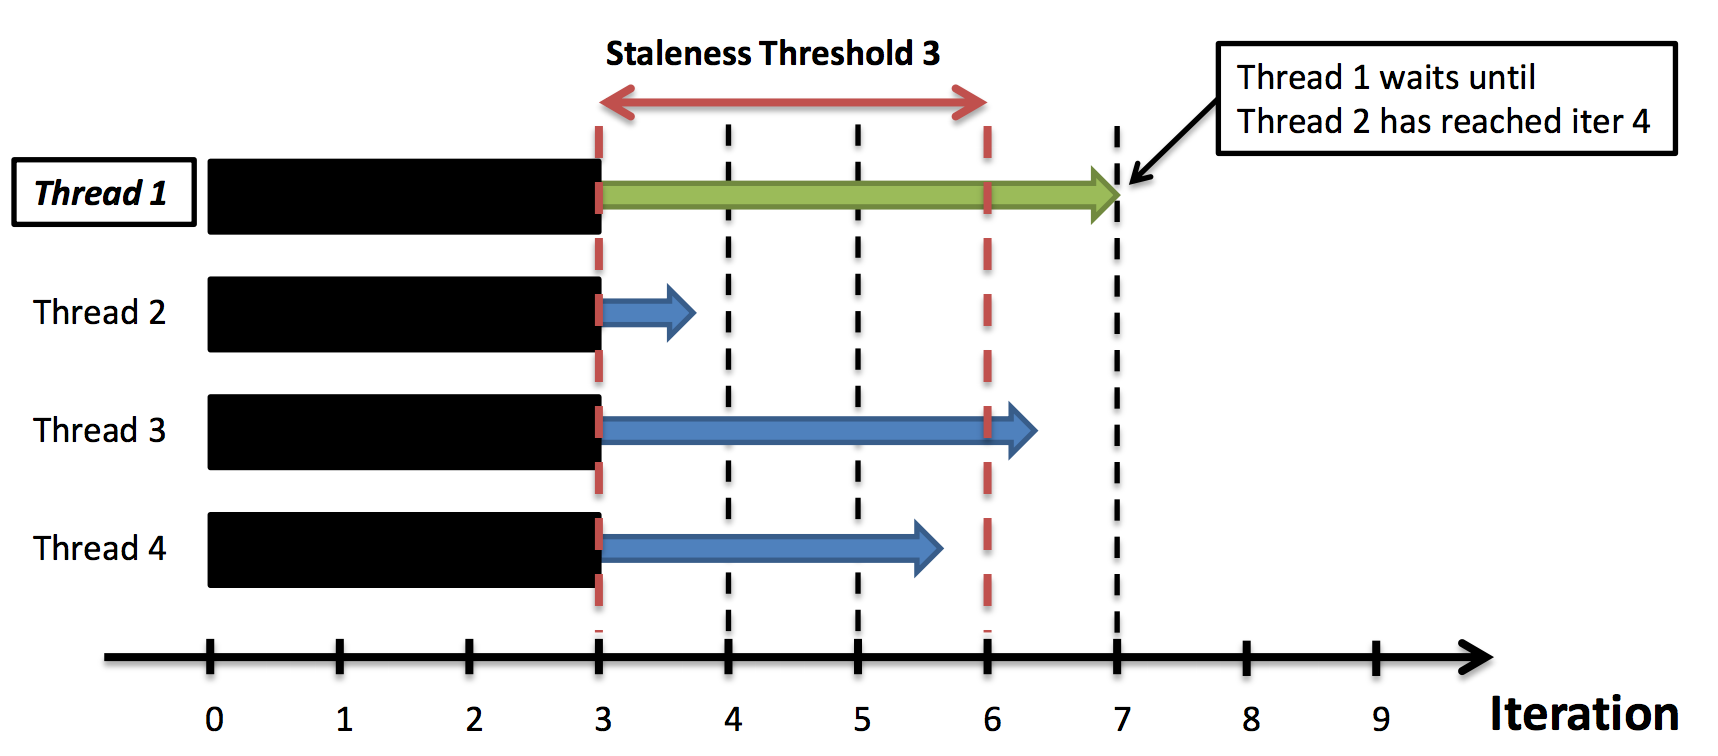
\includegraphics[width=0.8\linewidth]{SSP}
\caption{Stale Synchronous Parallel}
\label{fig:SSP}       % Give a unique label
\end{figure}

通常可以从两个方向着手缓解上述的挑战,第一个方向是通过更好的参数服务器实现和设计来提供更高效的服务;
另外一个方向是从算法应用的角度出发,通过更好的算法设计和参数服务器使用,来减少网络通讯和延迟。
前者的主要方式有压缩传输,Pipeline, SSP(Stale Synchronous Parallel, SSP)等等。
后者的主要方式包括从应用的角度减少参数的访问,使用更小更紧凑的参数类型,更稀疏的参数表示等等。为此,接下来本章将主要介绍如何设计分布式流式主题模型的参数存储和使用。


\section{流式主题模型词汇表}
在互联网环境下,流式数据没有尽头,人们无法提前预知数据的分布,因而数据流上不断会有未登录词出现。
我们知道词汇的分布服从幂率分布,也就说大语料中绝大多数出现的词汇属于低频词,并且在流式数据中呈现出线性增长的趋势,如图\ref{fig:power-law, fig:noFreq2-5VsWords}。

\begin{figure}[htb]\centering
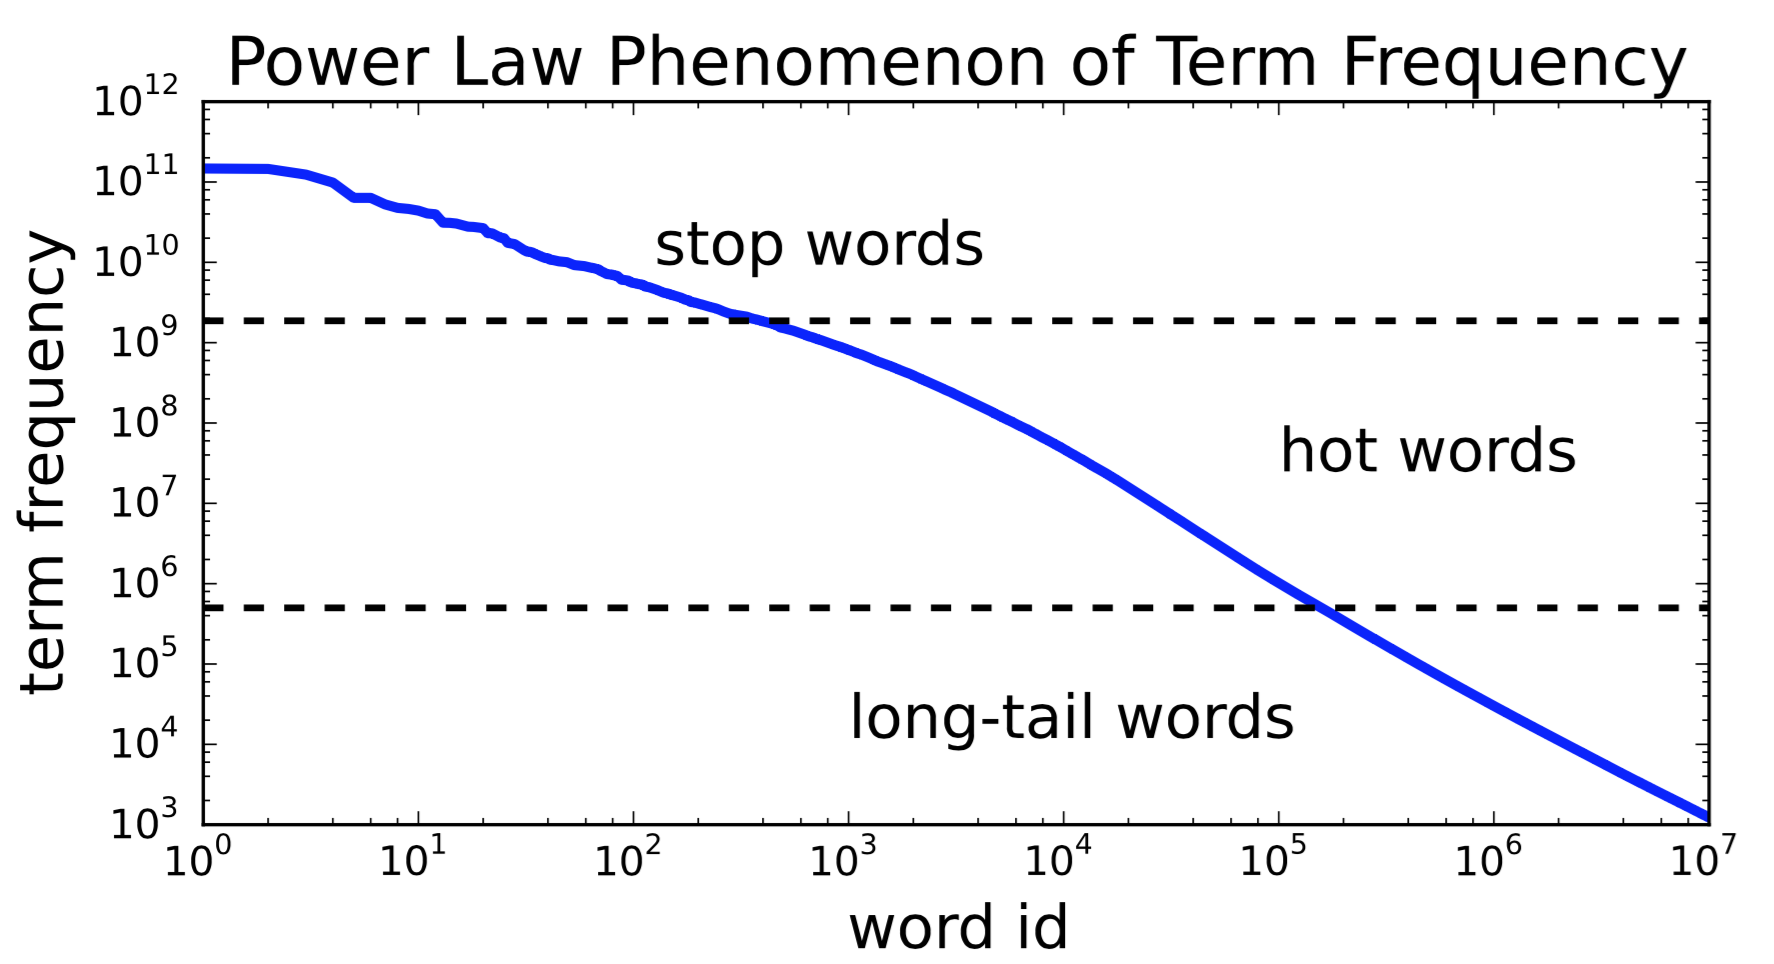
\includegraphics[width=0.5\linewidth]{power-law}
\caption{词频的幂率分布现象}
\label{fig:power-law}       % Give a unique label
\end{figure}

图\ref{fig:power-law}来自于论文\cite{yuan2015lightlda}, 是分析150亿个网页得到的结果,显示除了少量的静态词之外(几百上千),中间大约有几万-几十万个常用词,其他的词汇属于低频词。
论文\cite{yuan2015lightlda}还提到静态词和常用词大约只占所有词汇的$10\%$,而低频词却占了$90\%$。然而,静态词和常用词大约覆盖了$95\%$的语料,而低频词仅仅占了$5\%$。

\begin{figure}[htb]\centering
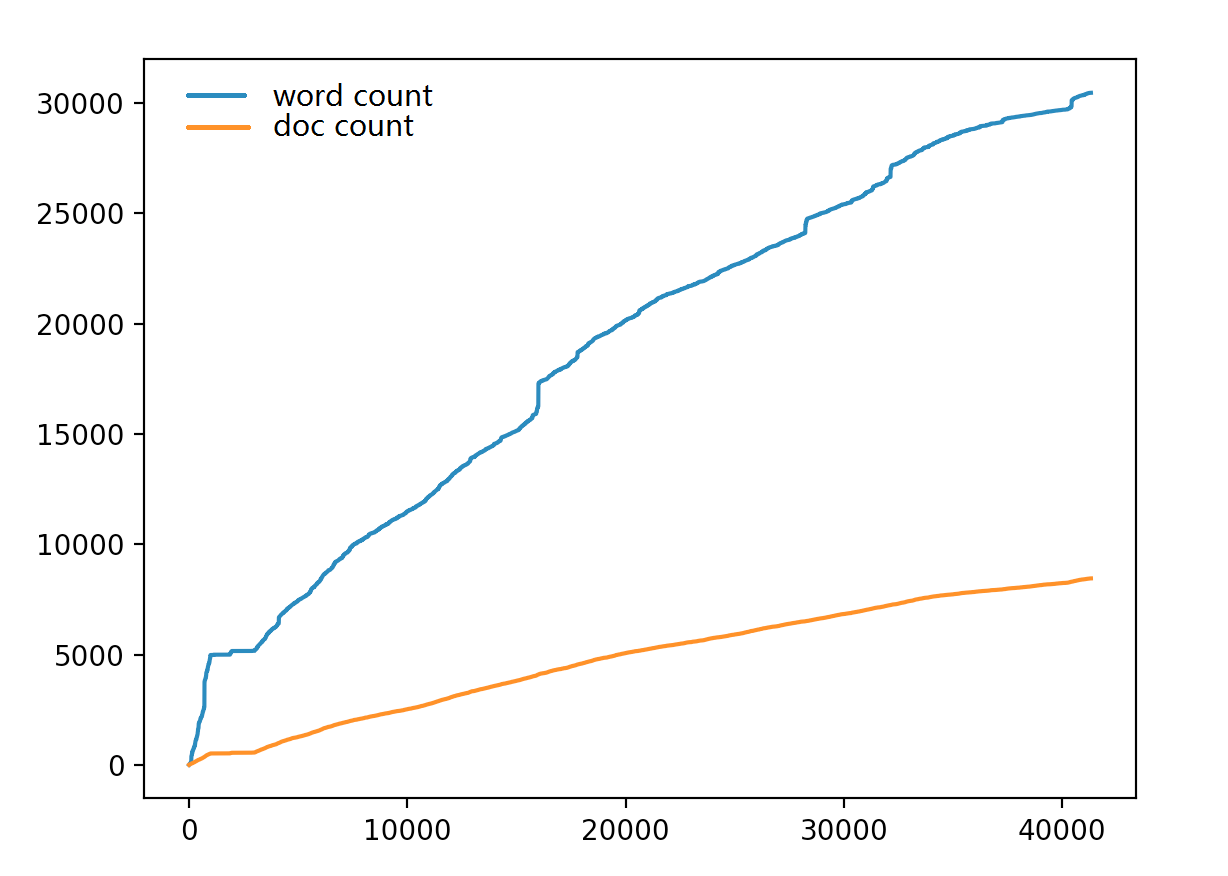
\includegraphics[width=0.5\linewidth]{noFreq2-5VsWords}
\caption{文档与低频词关系图}
\label{fig:noFreq2-5VsWords}       % Give a unique label
\end{figure}

图\ref{fig:noFreq2-5VsWords}中上方蓝色的线表示词频2-5的低频词随着文档数的增长趋势。下方的橙色线则表示包含这个区间内低频词的文档增长趋势。容易发现低频词的呈线性增长趋势。

通过前面章节的介绍,分布式主题模型的参数模型通常是一张词汇-主题计数表TAB(V, Z),表中的每一行对应着一个词汇的主题分布情况。在流式环境下,由于词表是动态增长的,这就意味着如果想要保留新增的词汇,那么我们必须维护一个动态词表。
因而维护一个动态词表的同时也要维护词汇-主题计数表TAB(V, Z)。
最简单的方式便是当词表中新增一个词汇时,相应地创建一个新的主题计数向量。
同理如果删除一个词汇也要相应地删除这个主题的计数向量。

根据上面的分析简单的动态词表维护策略,显然在实际应用中是行不通的。
这种做法将会遇到如下问题:

(1) 词表表超大,当主题个数超多时参数规模将会巨大无比。

(2) 维护动态词表,可能需要频繁的增删动态词表和词汇-主题计数表TAB(V, Z),这种维护代价有可能造成频繁的内存创建和回收,使得算法变得低效而无法被容忍。

解决和两个问题最为简单且行之有效的方法是使用先验知识提前设计一个静态的词表,这个词表里面只包含最经常被使用的一小部分词汇(根据前面的分析,仅需要涉及数十万个词汇即可)。
这种方法,避免了动态词表的维护,并且大大减少了参数规模,在许多主题模型的实现中都得到了应用。

\begin{figure}[htb]\centering
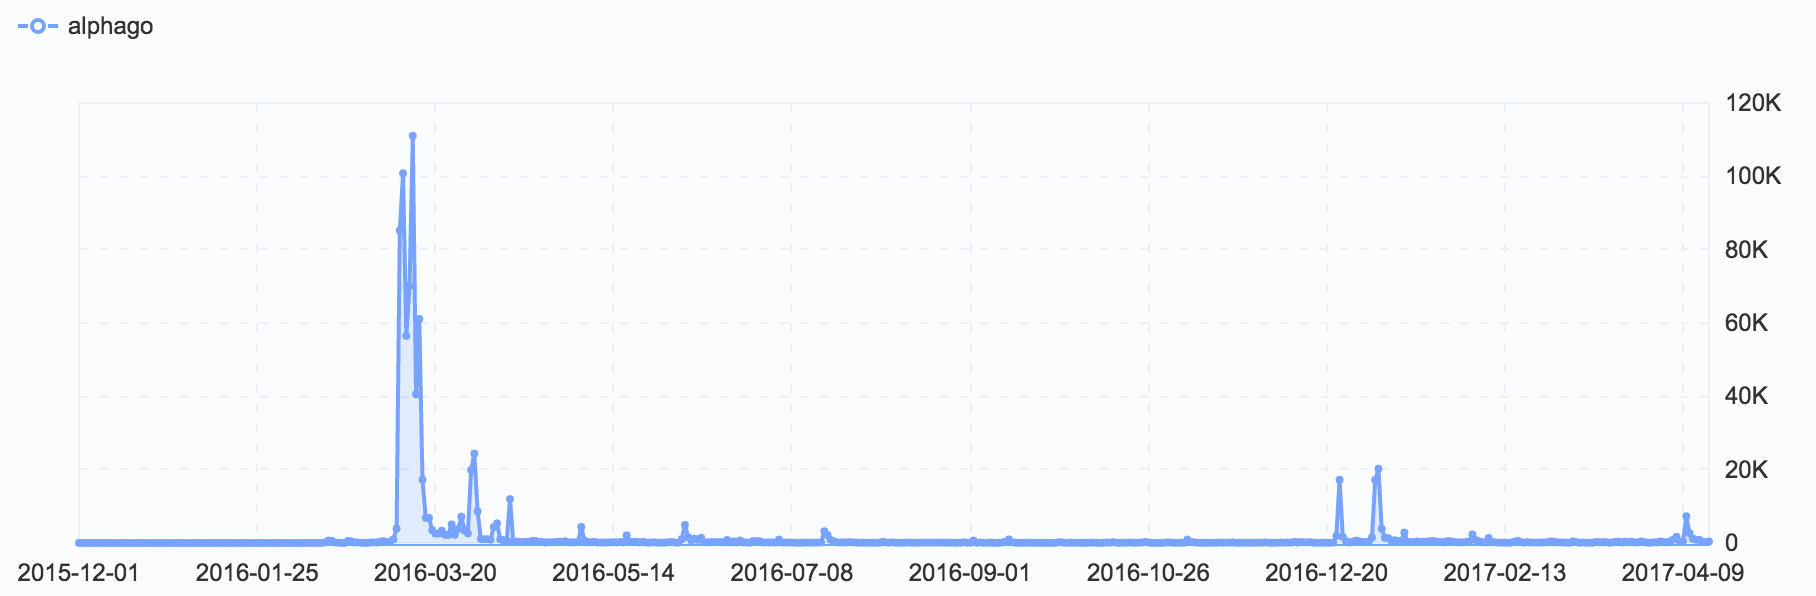
\includegraphics[height=0.23\linewidth,width=0.7\linewidth]{word-trend-alphago}
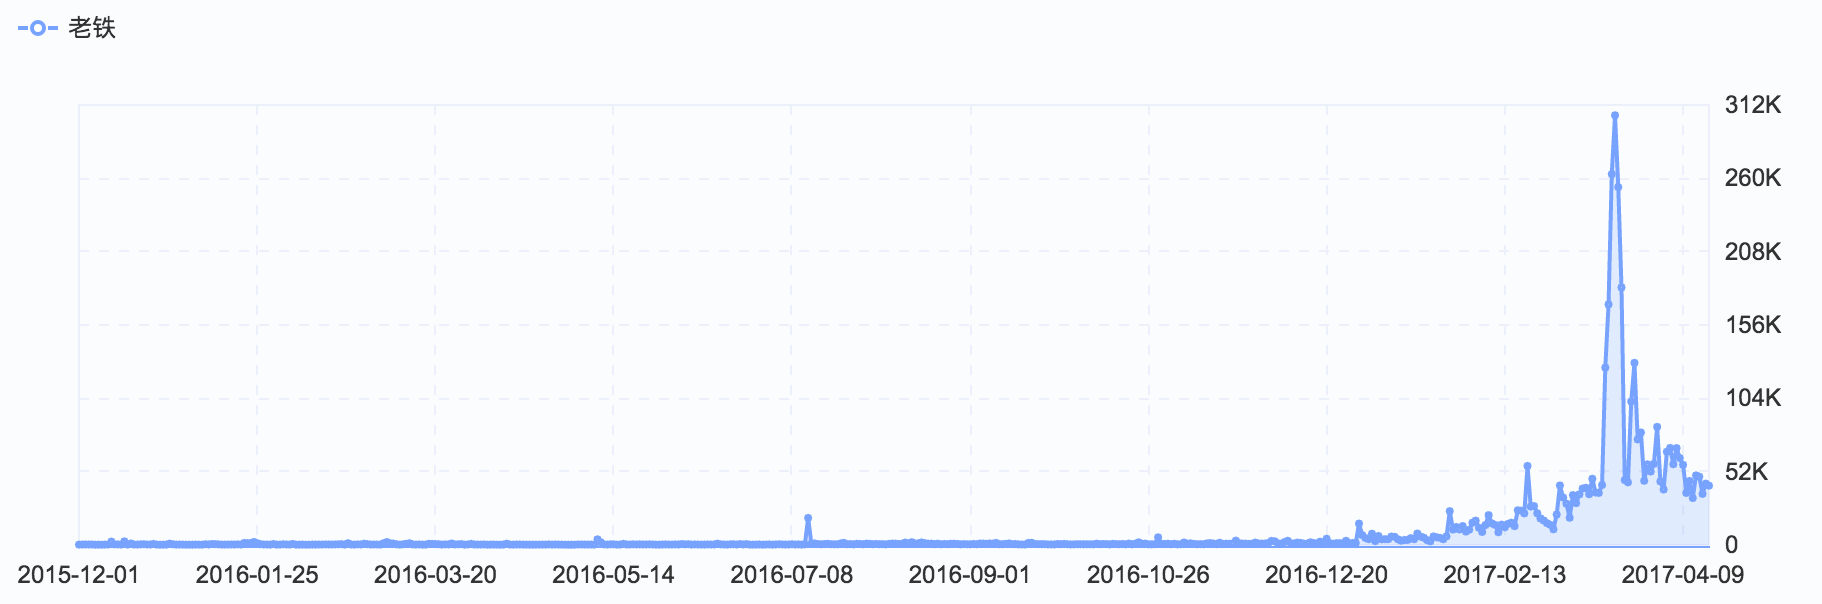
\includegraphics[height=0.23\linewidth,width=0.7\linewidth]{word-trend-laotie}
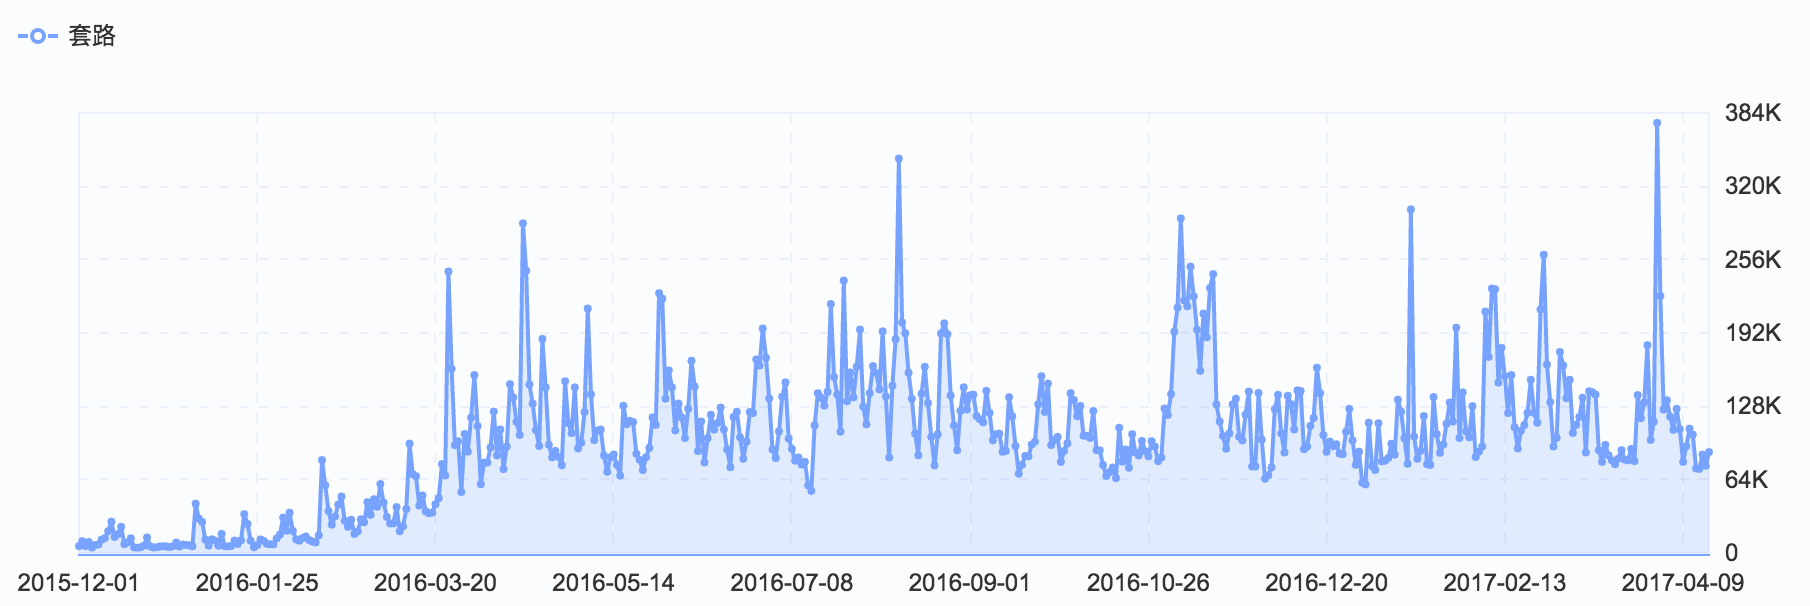
\includegraphics[height=0.23\linewidth,width=0.7\linewidth]{word-trend-taolu}
\caption{微博新词被提及的整体趋势}
\label{fig:new-word-trend}       % Give a unique label
\end{figure}

然而这种方法词表的规模很难确定,在不同的应用中主题模型可能需要不同阈值。
另外,固定大小的词汇表会使得许多有意义的词汇被忽略。
在流式数据中,由于词表是动态增长的,动态维护一个动态词表是有意义的。
因为社交网络的广泛应用和传播,使得许多新词被挖掘发现并得到追捧。图\ref{fig:new-word-trend}显示了今年来兴起的一些新词,类似的新词还有许多。

除此之外在具体的工业场景应用中,人们发现当数据量足够大且模型的主题个数足够多时,主题模型的效果会得到显著的提升。
这其中一个重要的原因是当数据量大时,许多覆盖低频词的主题语义被保留下来了\cite{Peacock}。
图\ref{fig:ntopics-pmi}显示了主题PMI分值,显然当主题个数越多时,PMI分值显著地提高了。

\begin{figure}[htb]\centering
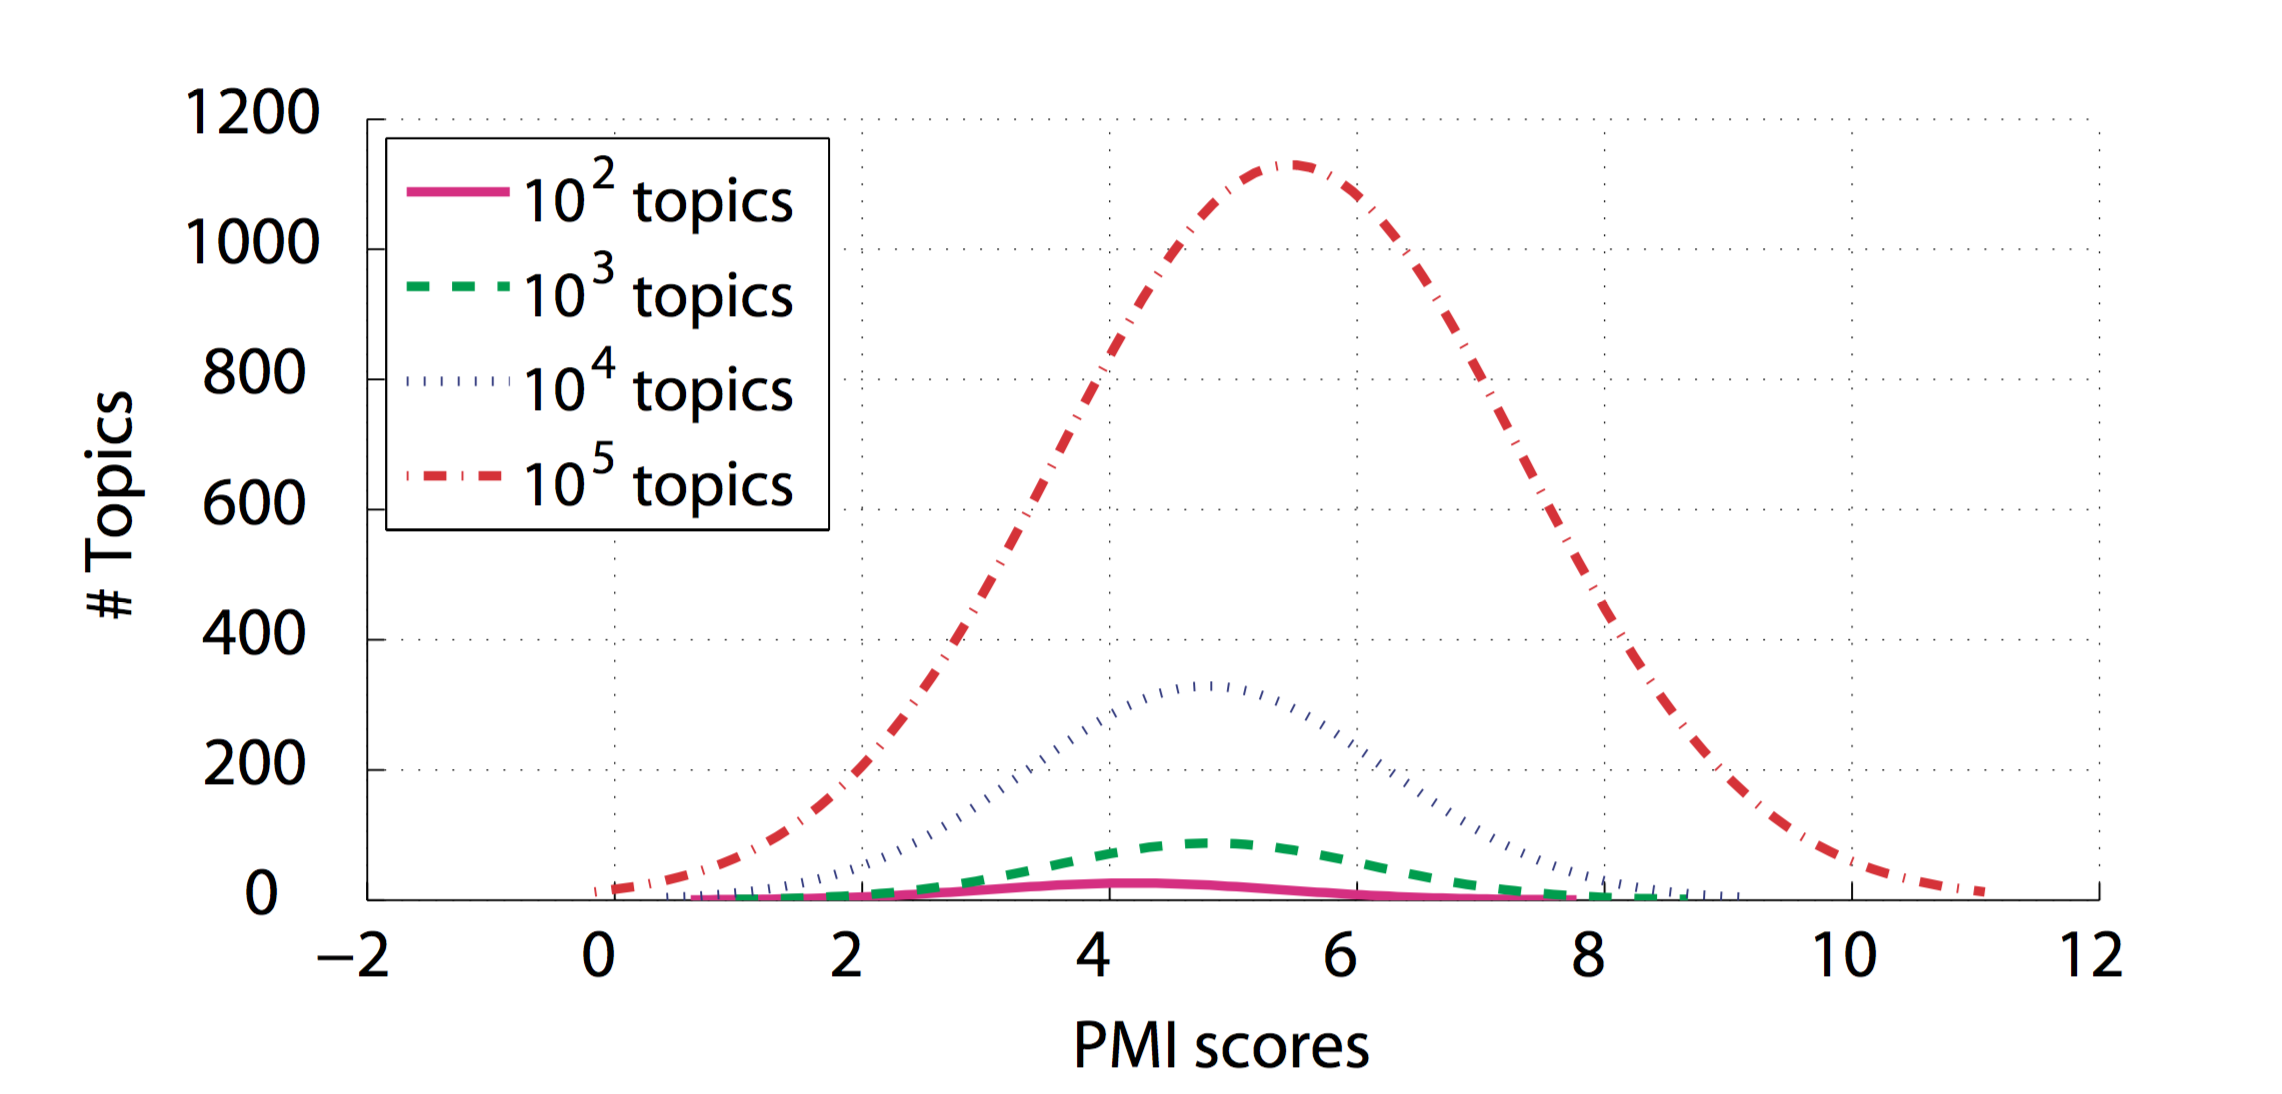
\includegraphics[width=0.7\linewidth]{ntopics-pmi}
\caption{LDA主题个数与PMI关系}
\label{fig:ntopics-pmi}       % Give a unique label
\end{figure}

这些分析都说明在流式数据上维护一个动态词表具有重要的意义。

实际上许多地方都提到了主题模型的词汇-主题表是一个特别稀疏的矩阵,对于大部分词汇来说,其语义是高度集中的,特别是低频词。
因而,如果采用稀疏表达的形式,比如哈希表,词汇-主题表的规模将大大减小。
然而完全使用稀疏表达也存在两个问题:

(1) 稀疏表达的矩阵或向量的随机访问效率不如稠密矩阵的高

(2) 当矩阵或向量相对稠密时,使用稀疏表达需要数倍于稠密的表达的空间消耗

上述的两个问题都会影响到主题模型算法的效率,其中第二个主要体现于在参数更新和访问过程中需要更多的网络传输。


\begin{figure}[htb]\centering
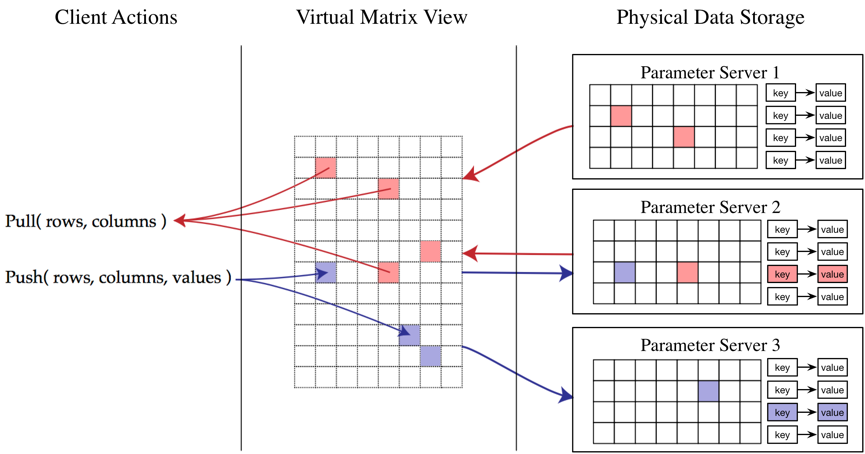
\includegraphics[width=0.8\linewidth]{hybrid-ps}
\caption{混合参数数据结构}
\label{fig:hybrid-ps}       % Give a unique label
\end{figure}

借助之前的分析结我们知道非低频词覆盖的数据大约占了$95\%$,也就是说在模型训练过程中有大量的参数访问来自于非低频词。
因而本文提出的解决方法是一种混合的参数数据结构。
这种混合数据结构既包含了稠密的表达,同时又包含了稀疏的表达。

在构建词汇表过程中,我们首先选取一个足够大的静态词汇表。
主要做法是选取一个相对较大的阈值筛选出了一部分高频词,针对这些词汇采用静态的词汇集表示,并构建<词汇, ID>映射。
剩余的词汇则采用动态的词汇表表示,由于数据流中不对会有新词出现,同时算法存在对过时的词汇的删除策略,因而动态词汇表时刻会产生变化。
所以,参数数据结构也会做出相应的修改。

如图\ref{fig:hybrid-ps},词汇-主题表所对应的参数结构按照词汇表的设计被划分成为了两个部分,其中一部分是静态的稠密矩阵表示,另外一部分则是使用<key, value>的形式进行稀疏的存储。

通过上面的设计方案,我们既高效地维护了一个动态词表,同时又使得绝大多数数参数访问和修改发生在了稠密矩阵上。

\section{优化实现方案}
除了上面通过优化参数数据结构的方案来提高算法的参数服务器的使用性能之外,
一些具体的实现技巧也能大大提高算法的效率,这种思路在许多高效的算法实现中都能看到。

\subsection{使用int和float基本类型}
在基本类型中,最经常使用的整型int和浮点型float都只占用4个字节,而long和double类型通常占用8个字节。
这些类型的值域分别是:

int $\sim [-2147483648, 2147483647]$,

float $\sim [-3.4E(+/-)38, 3.4E(+/-)38]$, 

long $\sim [-9223372036854775808, 9223372036854775807]$,
	 
double $\sim [-1.7E(+/-)308, 1.7E(+/-)308]$。

int和float所能表示的范围和精度有限,当数据太大时可能造成溢出。
然而当参数规模足够大时,使用4字节类型和使用8字节类型之间将会有成倍的存储效率差距。

但是根据图\ref{fig:power-law}显示,除了静态词很少会有词汇超过int所能表达的值域。而在主题模型中静态词通常会在训练之前被遭到过滤。因而如果使用long和double类型意味着很大的浪费。

在本文的实现中,我们选择了4字节基本类型作为参数类型。

\subsection{优化算法采样顺序}

\begin{algorithm}[htb]
\label{alg:natural-order}
\caption{Sample in Natural Order}
\begin{algorithmic}[1] 
\Require TAB(V, Z), $\mathbf{k} = [1, 2, ..., K], \mathbf{w}$
\For { m = 1 to $M$ }
\For { n = 1 to $N_m$}
\State \textbf{Require} parameter $n(w_{mn}, \mathbf{k}) \sim$ TAB(V, Z)
\State SAMPLE($z_{mn}, n(w_{mn}, \mathbf{k})$)
\EndFor
\EndFor
\end{algorithmic}  
\end{algorithm}  
常见的主题模型Gibbs采样算法是坐标轴下降方法,交替轮换坐标轴逐一地采样更新。
在一般情形中,对语料采样通常是语料中词汇出现的自然顺序,先后地对出现的词汇执行采样,如算法\ref{alg:natural-order}。

根据LDA模型Gibbs采样的概率分布公式,词汇采样过程中将会使用到与词汇关联的词汇主题分布$n(w, \mathbf{k})$。
但是自然顺序,词汇在语料中的分布式散乱的,前后被采样的词汇基本上是不相同的,相当于每次采样都随机地访问了词汇-主题表TAB(V, Z)中的一行。

这种情况下词汇主题分布向量$n(w, \mathbf{k})$难以被复用(做到这点必须完全加载整张表,而前面分析提到这张表有可能超过单机内存的容量)。
另外一方面,如果不复用$n(w, \mathbf{k})$,则需要频繁地对参数服务器发起pull请求,这显然会增加网络请求的次数,
不仅产生了更多网络延迟同时也更容易造成参数服务器的响应瓶颈,更严重的情况可能造成参数服务器崩溃或者网络通信失败。
显然,这种访问效率是极其低效的。

\begin{algorithm}[htb]
\caption{Sample in Vocabulary Order} 
\label{alg:vocab-order}
\begin{algorithmic}[1]
\Require TAB(V, Z) = \textbf{\{Dense(V, Z), Sparse(V, Z)\}}, $\mathbf{k} = [1, 2, ..., K], \mathbf{w_d, w_s}$
\Function{DO\_SAMPLING}{$\mathbf{n(v_b, k), w}$}
\For { each $t$ in $\mathbf{v_b}$}
\For { each $(m , n)$ where $w_{mn } = t$}
\State SAMPLE($z_{mn}, n(w_{mn}, \mathbf{k}), \mathbf{w}$)
\EndFor
\EndFor
\EndFunction
\For { each block $\mathbf{n(v_b, k)}$ in \textbf{Dense(V, Z)} }
\State Issue DO\_SAMPLING($\mathbf{n(v_b, k), w_d}$)
\EndFor
\State Set $\mathbf{v_s}$ as the low-frequent vocabulary local
\State Pull all $\mathbf{n(v_s, k)} \sim $ \textbf{Sparse(V, Z)}
\State Issue DO\_SAMPLING($\mathbf{n(v_s, k), w_s}$)
\end{algorithmic}  
\end{algorithm}  

实际上,Gibbs采样算法并没有严格要求采样的顺序。
根据主题模型参数数据结构的设计,令TAB(V, Z) = \{Dense(V, Z), Sparse(V, Z)\},
其中Dense(V, Z)表示稠密的参数矩阵,Sparse(V, Z)表示稀疏的<Key, Value>参数矩阵。

Dense(V, Z)所对应的词汇子集都是高频词,这些词汇在所有语料子集上都有很大的概率会出现。
根据这些特性,按块读取稠密矩阵Dense(V, Z),虽然有可能会下载一些无用的参数,但是将会大大提高网络传输的效率。

Sparse(V, Z)所对应的词汇子集含有大量的低频词,大部分词汇不大可能出现在所有的语料子集上。因而每个子集上的低频词词汇表只是全局低频词词汇表的一个较小的子集
。因为这部分参数高度稀疏,所以实际中可以完整下载本地所有需要的参数。

根据以上的参数数据结构特性,本文算法\ref{alg:vocab-order}实现中将文档分为高频词和低频词两部分。
之后对高频词部分按照词汇表顺序排序汇总。
同时对静态稠密的Dense(V, Z)参数矩阵进行分块。

当采样算法开始时,算法实现按照块读取的方式读取Dense(V, Z)参数稠密矩阵的一部分,并在语料文档中的稠密部分执行相应词汇的重采样。
执行完改步骤之后,从Sparse(V, Z)中pull将本地所有本地需要的低频词参数,并执行文档低频词部分的重采样。

\subsection{Pipeline参数更新}
当Gibbs采样是按照文本语料中词汇的自然顺序采样时,参数不得不等待所有语料中词汇都被采样之后在同步更新。
这种做法在采样过程中网络处于空闲状态,而在参数更新时又很容易出现网络使用高峰。

在按照上一小节的方式优化Gibbs采样顺序之后,我们发现每个词汇的主题分布向量无需互相等待,因而在一个词汇所有出现位置都经过采样之后便可以执行参数的增量更新。
这种方法称之为Pipeline,它将参数在时间维度上异步均摊地执行网络更新,不仅在采样过程中利用了网络,还有效地解决了网络高峰的问题。

\begin{figure}[htb]\centering
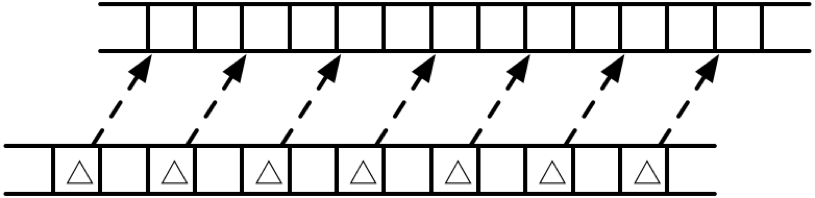
\includegraphics[width=0.7\linewidth]{pipeline}
\caption{Pipeline异步地进行网络传输}
\label{fig:pipeline}       % Give a unique label
\end{figure}


\begin{algorithm}[htb]
\caption{Pipeline Parameters Update} 
\label{alg:vocab-order}
\begin{algorithmic}[1]
\Require TAB(V, Z) = \textbf{\{Dense(V, Z), Sparse(V, Z)\}}, $\mathbf{k} = [1, 2, ..., K], \mathbf{w_d, w_s}$
\Function{DO\_SAMPLING}{$\mathbf{n(v_b, k), w}$}
\For { each $t$ in $\mathbf{v_b}$}
\For { each $(m , n)$ where $w_{mn } = t$}
\State GibbsSampling($z_{mn}, n(w_{mn}, \mathbf{k}), \mathbf{w}$)
\EndFor
\State Calculate update $\Delta \beta(w, \mathbf{k})$
\State Push $\Delta \beta(w, \mathbf{k})$ to parameter
\EndFor
\EndFunction
\For { each block $\mathbf{n(v_b, k)}$ in \textbf{Dense(V, Z)} }
\State Issue DO\_SAMPLING($\mathbf{n(v_b, k), w_d}$)
\EndFor
\State Set $\mathbf{v_s}$ as the low-frequent vocabulary local
\State Pull all $\mathbf{n(v_s, k)} \sim $ \textbf{Sparse(V, Z)}
\State Issue DO\_SAMPLING($\mathbf{n(v_s, k), w_s}$)
\end{algorithmic}  
\end{algorithm}  

\subsection{稀疏参数矩阵的维护}
在本文主题模型参数数据结构的设计中,低频词-主题分布表Sparse(V, Z)的稀疏性起到了至关重要的作用。
但是如果没有得到维护,也会显现出一些问题。本节主要介绍流式环境下如何维护Sparse(V, Z)稀疏矩阵。

在上一章,本文介绍了两个流式主题模型算法框架,分别是在线流式主题模型\ref{alg:onlineStreamLDA}和增量流式主题模型\ref{alg:IncStreamLDA}。

实际上在线流式主题模型中,参数$\beta^{(t)}(w, k) = (1 - \rho_t) \beta^{(t-1)}(w, k) + \rho_t n_{k, w}^{(t)}$是一个加权平均值。其中$\rho_t \in (0, 1)$,说明几轮迭代之后,$\beta^{(t)}(w, k)$将会出现很多小数值。
假设$\beta^{(t-\sigma)}(w, k) = 1$,并且在其后的$\sigma$轮迭代中都有$n_{k,w} = 0$,
那么$\beta^{(t)}(w, k) = (1 - \rho_t)^{\sigma} > 0 $。
我们发现$\beta^{(t)}(w, k)$将会变得较小,但是不会变为0。
换句话说,$\beta^{(t)}$矩阵中将会出现大量的非零元,Sparse(V, Z)的稀疏性会大大降低,带来的是存储空间的消耗和更多的网络传输。

然而$\beta^{(t)}$中的绝大多数非零元对LDA Gibbs采样概率分布的影响微乎其微。
为了保证$\beta^{(t)}$的稀疏性,本文提出了两种做法:

(1) 设置阈值,对较小的小数进行截断。比如,如果$\beta^{(t)}(w, k) < 0.05$,删除该非零元。

(2) 采用int类型存储$\beta^{(t)}$,在每轮迭代的执行加权平均时使用四舍五入的方法转为整型。

相对于在线流式主题模型,增量主题模型只有增量的更新操作,并且每次更新都是一个整型值,所以更适合于参数服务器的使用模式(增量地更新)。
另外,因为增量流式主题模型设置了窗口大小,所以模型中参数值$\beta(w, k)$最终稳定在某一个范围区间内。
同时,随着模型的逐渐收敛,$\beta^{(t)}$中的元素会出现越来越多的零元。

以上两个算法都需要单独的步骤来删除稀疏数据结构Sparse(V, Z)中的零元来提高非零元的存储比例,减少不必要的网络传输。


\section{实验分析}

\subsection{静态词表实验分析}
\begin{figure}[htb]\centering
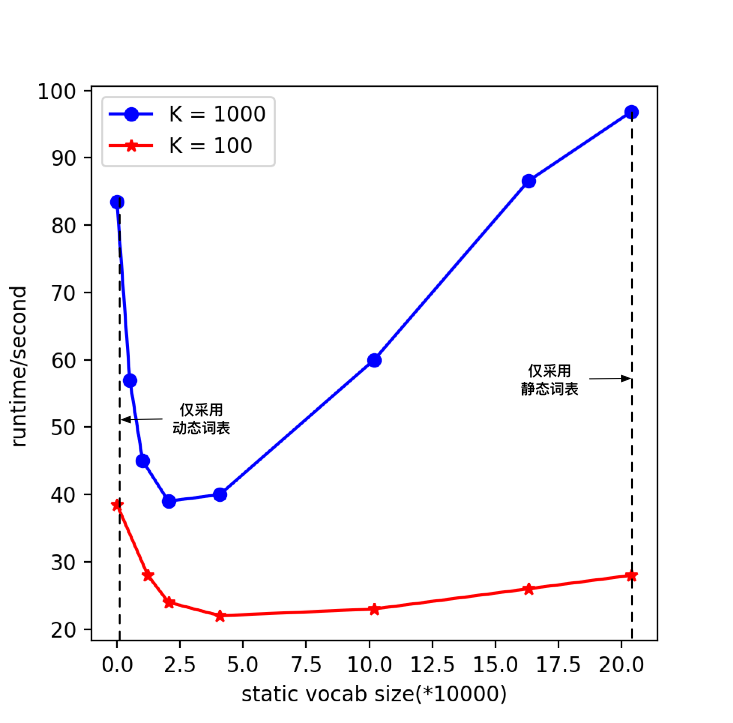
\includegraphics[height=0.41\linewidth]{static-vocab-vs-runtime}
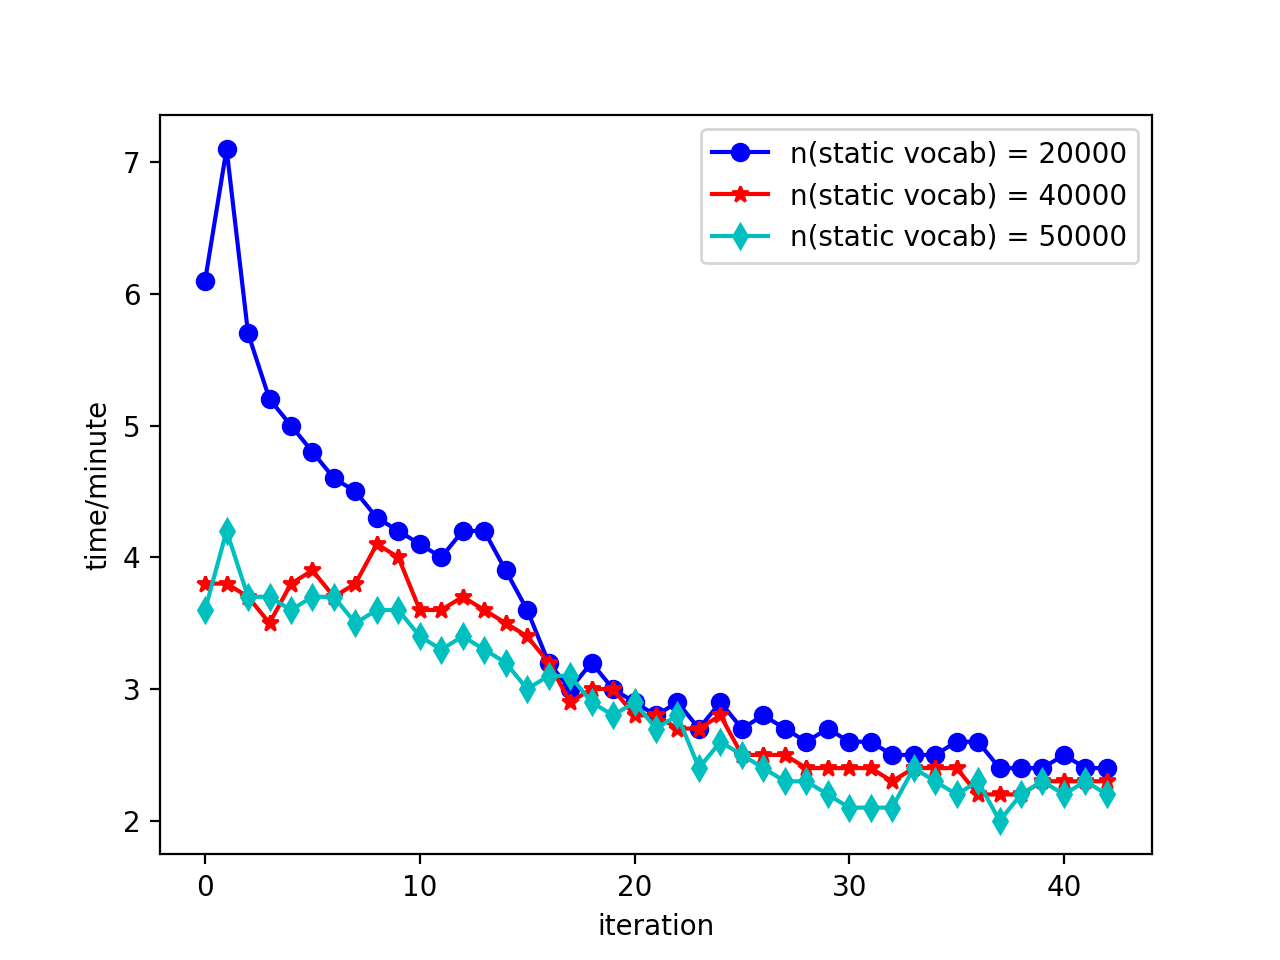
\includegraphics[height=0.41\linewidth]{static-vocab-runtime-iteration}
\caption{静态词表大小与运行时间关系示意}
\label{fig:static-vocab-runtime}       % Give a unique label
\end{figure}

图\ref{fig:static-vocab-runtime}所显示的是静态词表大小与算法运行时间之间的关系。

在左子图中,实验中每轮迭代遍历41310个文档,语料中出现的词汇总量为203891。
左子图中显示的纵坐标运行时间为算法采样10轮的时间平均值(单位为秒),横坐标表示的静态词汇表的大小(*10000)。
本文分别统计了主题维度为100和1000两种情况下,算法运行时间与静态词汇表大小之间的关系。
如图所示,我们不难发现曲线呈对钩形状。在这个实验中静态词汇表的带下设置为50000左右比较合适。
静态词汇表太大,低频词会逐渐增多,意味着混合参数中的Dense(V,Z)表会变得越来越稀疏,因而会大大降低算法的性能。
另外一方面静态词汇表也不能太小,语料中高频词的覆盖率占了绝大多数,小的静态词汇表无法充分地覆盖语料,使得许多参数访问被转向Sparse(V,Z),从而也会降低算法的性能。

在右子图中,实验中每轮迭代遍历808301个文档,语料中出现的词汇总量为982101。
纵坐标表示每轮迭代的运行时间(单位为分钟),横坐标表示算法的迭代轮数。
如果所示,本文分别设置了三组静态词表大小(20000,40000,50000),主题模型的维度都为1000。
不管静态词表的大小如何,随着迭代轮数的增长,运行时间都表现出下降的趋势。
起初三组实验算法运行时间存在明显的差异,其中静态词汇表大小为20000的实验显示运行时间远大于另外两组。
但是随着时间的推移,运行时间逐渐降低并且逼近另外两组。这是因为Sparse(V, Z)随着算法迭代轮数的增加越来越稀疏,带来了网络传输量的急剧下降。

\subsection{网络传输效率实验}

\subsection{采样算法效率实验}

\subsection{流式主题模型效果}

\section{本章小结}
